\documentclass[11pt]{article}

\usepackage{amsmath,graphicx}
\usepackage{amssymb,amsthm,bm,url,paralist,tabls,hyperref,amscd,appendix}


\newtheorem{thm}[equation]{Theorem}
\newtheorem{prop}[equation]{Proposition}
\newtheorem{lem}[equation]{Lemma}
\newtheorem{cor}[equation]{Corollary}
\newtheorem{conj}[equation]{Conjecture}
\newtheorem{rem}[equation]{Remark}
\newtheorem{examp}[equation]{Example}
\newtheorem{defn} [equation]{Definition}
\theoremstyle{remark}	  \newtheorem*{remark}{Remark}



\numberwithin{equation}{section}
\usepackage{varioref}
\labelformat{section}{Section~#1}
\labelformat{subsection}{Section~#1}
\labelformat{subsubsection}{Section~#1}
\labelformat{figure}{Figure~#1}
\labelformat{table}{Table~#1}
\labelformat{defin}{Definition~#1}
\usepackage[letterpaper,margin=1in]{geometry}

\title{Training Support Vector Machines with Weighted Reduced Convex Hulls}
\author{Mohammed Modan \\  Department of Mathematics, Statistics, and Computer Science \\  Macalester College \\   St. Paul, MN 55105
}



\date{December 19, 2017}

\begin{document}




\maketitle

\begin{abstract}
\noindent
In this paper, we show that for any knot $K$ there exists an orientable surface $S$, with boundary, such that the boundary of $S$ is isotypic to the knot $K$.  Our method is to study an algorithm due to Seifert, which produces such a knot.  We illustrate Seifert's algorithm with several examples, including the trefoil, the figure-8, and the knots denoted by 5-3 and 6-2 in  the Rolfsen atlas of knots. We also carefully go through the proof of Gabail, which says that Seifert's algorithm gives a genus-minimizing spanning surface for alternating knots.

 \end{abstract}


\section{Introduction}

Machine learning has come to run the world. From recommender systems to predictive analytics, machine learning is integrated into almost every interaction we make with technology. Machine learning can be either supervised or unsupervised. In the latter case, the algorithm is not told what to look for and discovers patterns in the data. For the former, data is preclassified and the algorithm can find patterns associated with the class provided. These algorithms, broadly, fall into either numeric predictors or classifiers. At a basic level, they operate as follows:

\begin{itemize}
	\item Train a model on input data with a known output
	\item The model can now predict an output from a new input
\end{itemize}

Algorithms can range from the relatively simple, like Naive Bayes, to the complicated and cutting edge, like neural networks. Each algorithm has its place and application in which the model will excel, and engineers/data scientists will capitalize on this fact to build their software accordingly to exploit the strengths of these algorithms. For example, Naive Bayes is frequently used for sentiment analysis or spam filtering. Support Vector Machines (SVMs) are commonly used in hand writing recognition and protein classification due to its versatility.

SVMs typically perform very well while simultaneously avoiding overfitting data. Unfortunately, SVMs come with their drawbacks as well. They may not perform as well with very noisy data, and along with other complex machine learning algorithms such as neural networks, SVMs can be difficult to interpret and they are often seen as a "black box." When explaining the algorithm is necessary for a client, simpler algorithms such as decision trees or logistic regression are typically used which are simple to interpret.

\section{What is an SVM?}

A Support Vector Machine (SVM) is indeed a type of machine learning algorithm. In order to understand their method of function, however, it is necessary to understand the format of the data. Columns of a dataset can be considered variables, and rows as observations. Each row additionally has an associated class. Each row can be viewed as a point with an associated class in ${\rm I\!R}^{v}$ where $v$ equals the number of variables. For example consider the \texttt{iris} dataset in R (\ref{table:iris}). Each row is a point in ${\rm I\!R}^{2}$.

\begin{table}[h]
\centering
\begin{tabular}{c c | c}
Petal Length  & Petal Width & Species \\
\hline
1.4 & 0.2 & setosa  \\
1.4 & 0.3 & setosa  \\
1.3 & 0.2 & setosa  \\
4.7 & 1.4 & versicolor \\
4.5 & 1.5 & versicolor \\
4.9 & 1.5 & versicolor  \\
\end{tabular}
\caption{The \texttt{iris} dataset in ${\rm I\!R}^{2}$}
\label{table:iris}
\end{table}

Notice that these points can be plotted in ${\rm I\!R}^{2}$, coloring them by an arbitrarily assigned positive or negative class. Observe that this may give rise to class separation in the Cartesian plane. As illustrated in \ref{fig:margin}, a vector $w$ can then span between convex hulls of the positive and negative classes. The margin is defined as the norm of $w$, and the hyperplane separating the hulls is the perpendicular bisector of $w$. Note that an infinite number of $w$ can be drawn to separate the data, however there exists one unique hyperplane which maximizes the margin and maximizes separation. This occurs when $w$ spans the closest points between the convex hulls, as it does in \ref{fig:margin}. This $w$ defines the maximum margin and therefore maximally separating hyperplane.

\begin{figure}[!htbp]
$$
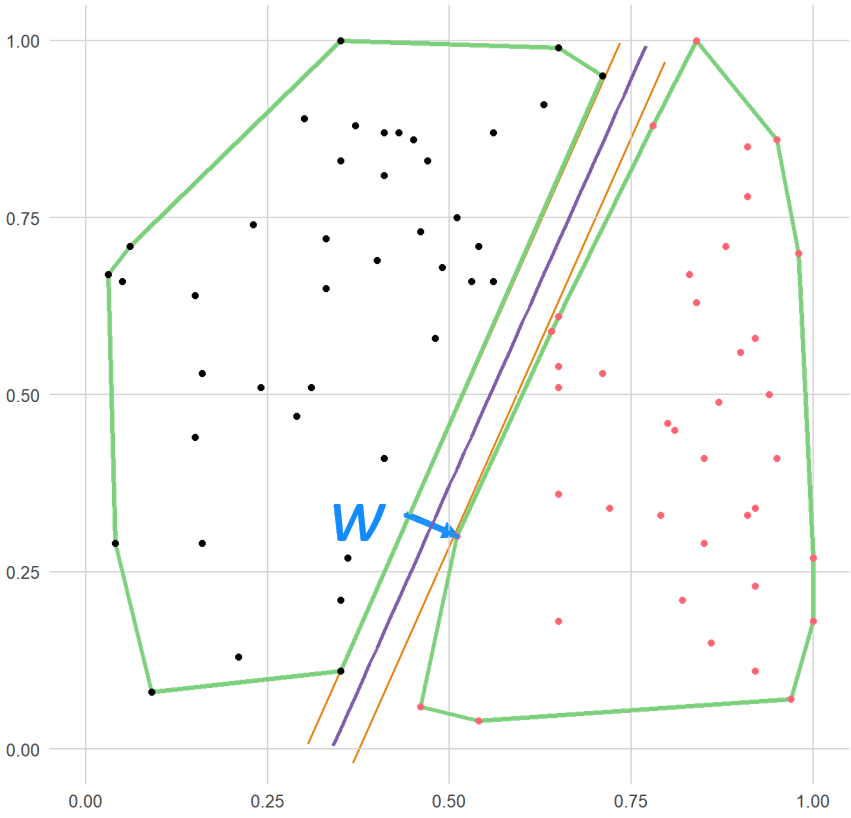
\includegraphics[width=4in]{Figs/hullPlane.PNG} 
$$
\caption{A dataset in ${\rm I\!R}^{v}$ with associated positive (salmon) and negative (black) classes. $w$ indicates the vector spanning the shortest distance between convex hulls of the classes (green), pointing to the positive class, defining the maximum margin (orange) hyperplane (purple) as its perpendicular bisector}
\label{fig:margin}
\end{figure}

Therefore we can define an SVM as follows:

\begin{defn}  An \emph{SVM} is a classifier defined by a maximally separating hyperplane.
\end{defn}

\section{Gabai's Theorem}

The genus of a knot $K$, denoted $g(K)$, is defined to be the minimum genus among all spanning surfaces for $K$.  When we construct a Seifert surface we produce a knot of some genus $\mathsf{g}$, which tells us that $g(K) \le \mathsf{g}$.  We will say that a spanning surface of minimum genus is \emph{genus-minimizing}.   An amazing Theorem of Gabia tells us that, for alternating knots, the surface produce by Seifert Algorithm from the previous section is genus minimizing.

\begin{thm} (Gabai \cite{Ga} 1986) If $K$ is an alternating knot and  $S$ is the spanning surface of $K$ produced by Seifert's algorithm then then $S$ is a genus-minimizing surface for $K$.
\end{thm}

\begin{proof} here is where we put the proof
\end{proof}


\appendix

\section{Code}

If you would like to include code from your project, place it in an appendix.

\bibliography{ExportedItems}
\bibliographystyle{ieeetr}
\end{document}


